\begin{multicols*}{2}
\section*{13. Thermal Radiation Heat Transfer}
\subsection*{13.1. General Procedure}
Most questions will ask for irradiation given some geometry and temperatures.
\begin{enumerate}
    \item Determine view factors $F_{ij}$ from inspection using the geometry.  Check for special cases such as:
    \begin{itemize}
        \item $F_{ii} = 0$ when the surface $i$ is planar or convex
        \item $F_{ij} = 1$ when the surface $i$ is a concave and fully encloses surface $j$
    \end{itemize}
    \item Check Figures section for view factors that cannot be obtained from inspection
    \item Use the reciprocity relation and summation rule to find the remaining view factors
\end{enumerate}
Solvability condition: Given $N$ surfaces, there are $N^2$ view factors. $N(N-1)/2$ view factors must be 
given by inspection, problem statement, or tables. The rest can be determined using reciprocity and summation.
\subsection*{13.2. Variable Definitions}
\begin{itemize}
    \item $F_{ij}$: View factor, the fraction of radiation leaving surface $i$ that strikes surface $j$ 
    \item $\omega$: Solid angle
    \item $G$: Irradiation, the rate of radiant energy incident on a surface per unit area
    \item $I$: Intensity
    \item $J$: Radiosity, the total rate of radiant energy leaving a surface per unit area
    \item $E_{b}$: Black body emissive power
    \item $\dot{Q}$: Heat transfer rate
    \item $\alpha$: Absorptivity
    \item $\rho$: Reflectivity
    \item $\tau$: Transmissivity
    \item $\epsilon$: Emissivity
    \item $\sigma$: Stefan-Boltzmann constant
\end{itemize}
\subsection*{13.3. Formulas}
Reciprocity relation:
\begin{align*}
    A_{1, s} F_{12} &= A_{2, s} F_{21} 
\end{align*}
Summation rule:
\begin{align*}
    \sum_{j=1}^n F_{ij} &= 1 
\end{align*}
Crossed-strings method:
\begin{figure}[H]
    \centering
    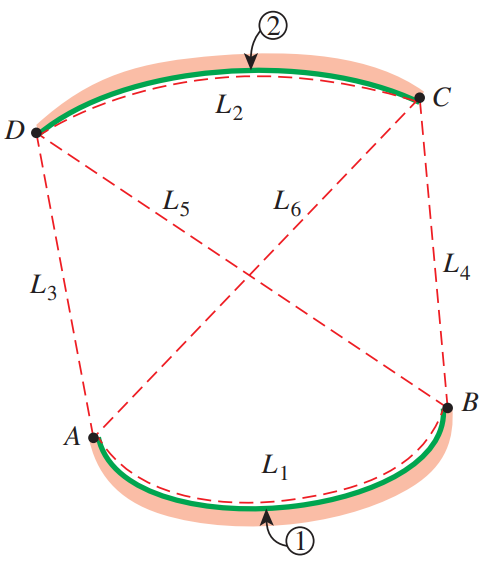
\includegraphics[width=0.2\textwidth]{Figures/Sec13 crossed strings.png}
    \caption{Determination of the view factor $F_{12}$ by the application of the crossed-strings method.}
    \label{fig:sec13_crossed_strings}
\end{figure}
\begin{align*}
    F_{12} &= \frac{(L_5 + L_6) - (L_3 + L_4)}{2 L_1} 
\end{align*}
On a black body, net radiation heat transfer is
\begin{align*}
    E_{bi} &= \sigma T_i^4 \\
    \dot{Q}_{12} &= A_{1, s} F_{12} \sigma (T_1^4 - T_2^4) = A_{2, s} F_{21} \sigma (T_1^4 - T_2^4) 
\end{align*}
On a grey body ($\epsilon_i = \alpha_i$, $\tau = 0$, $\alpha_i + \rho_i =1$), net radiation heat transfer is
\begin{align*}
    J_i &= \pi I_i = \epsilon_i \sigma T_i^4 + \rho_i G_i \\
    \dot{Q}_{12} &= \frac{A_{i, s} \epsilon_{i}}{1 - \epsilon_i} (E_{bi} - J_i) 
\end{align*}
For radiation in two-surface enclosures, net radiation heat transfer is
\begin{align*}
    \dot{Q}_{12} &= \dot{Q}_{1} = -\dot{Q}_{2} \\
    \dot{Q}_{12} &= \frac{\sigma (T_{1}^4 - T_{2}^4)}{\frac{1- \epsilon_1}{\epsilon_1 A_{1, s}} + \frac{1}{A_{2, s} F_{12}} + \frac{1-\epsilon_2}{\epsilon_2 A_{2, s}}} \\
    &= \frac{E_{b1} - E_{b2}}{R_{1} + R_{12} + R_{2}} 
\end{align*}
For some familiar geometries, the above equation simplifies, which is given in Table \ref{tab:sec13_radiation_enclosure_relations}.
\end{multicols*}

\section*{Figures}
\label{sec:sec13_figures}
\begin{figure}[H]
    \centering
    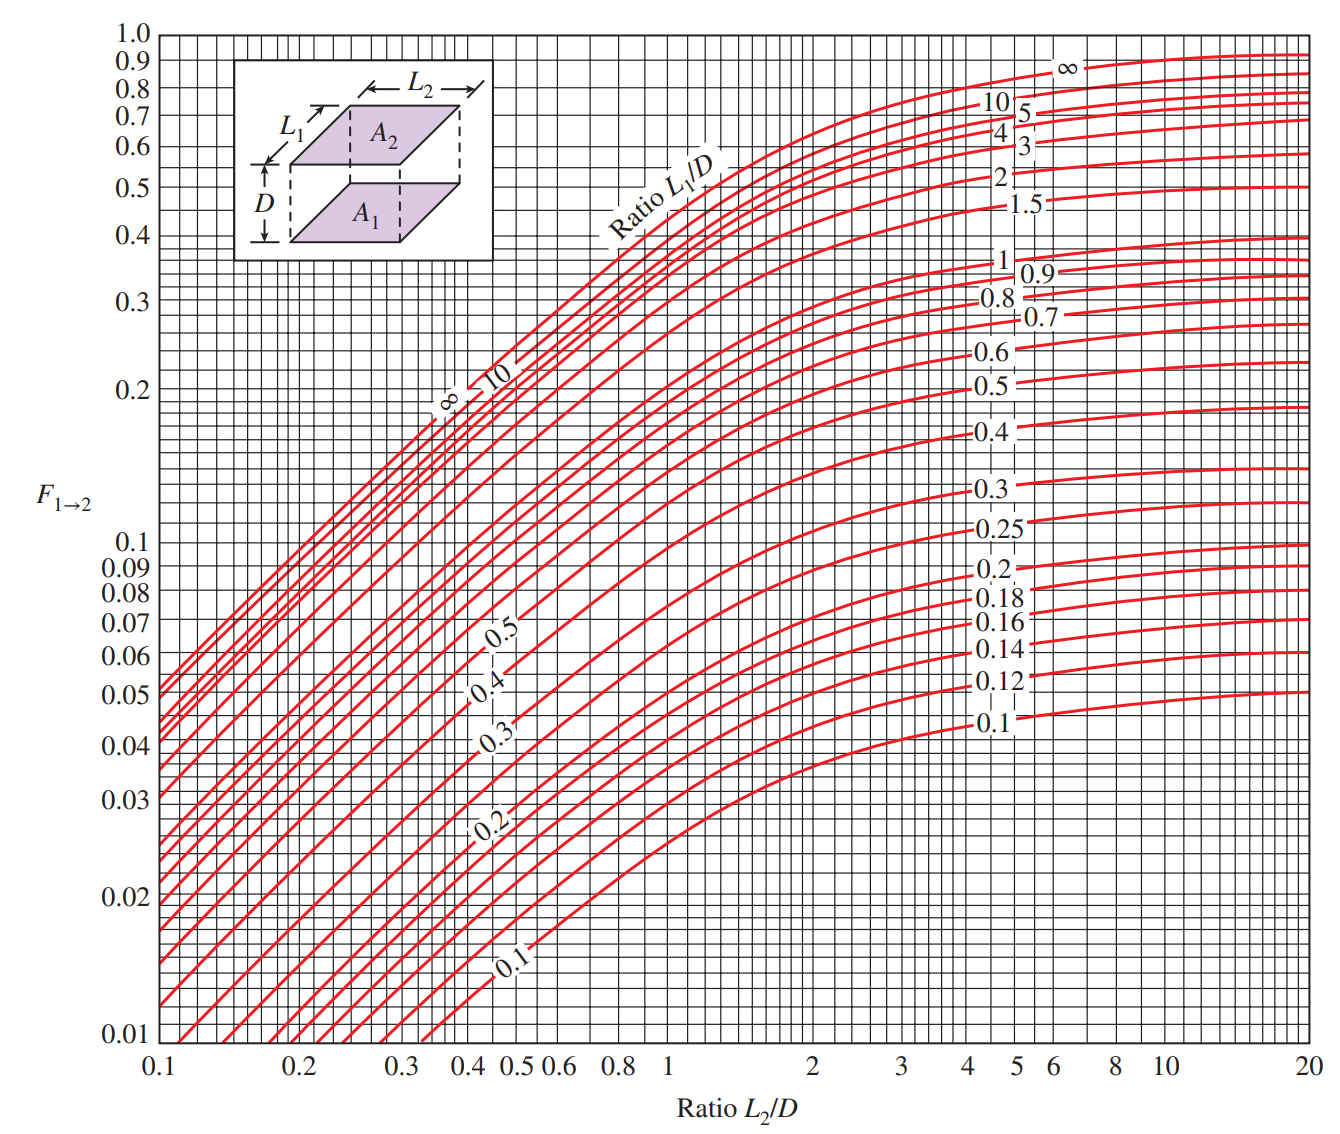
\includegraphics[width=0.6\textwidth]{Figures/Sec13 aligned parallel plates.png}
    \caption{View factor between two aligned parallel rectangles of equal size}
    \label{fig:sec13_aligned_parallel_rectangles}
\end{figure}
\begin{figure}[H]
    \centering
    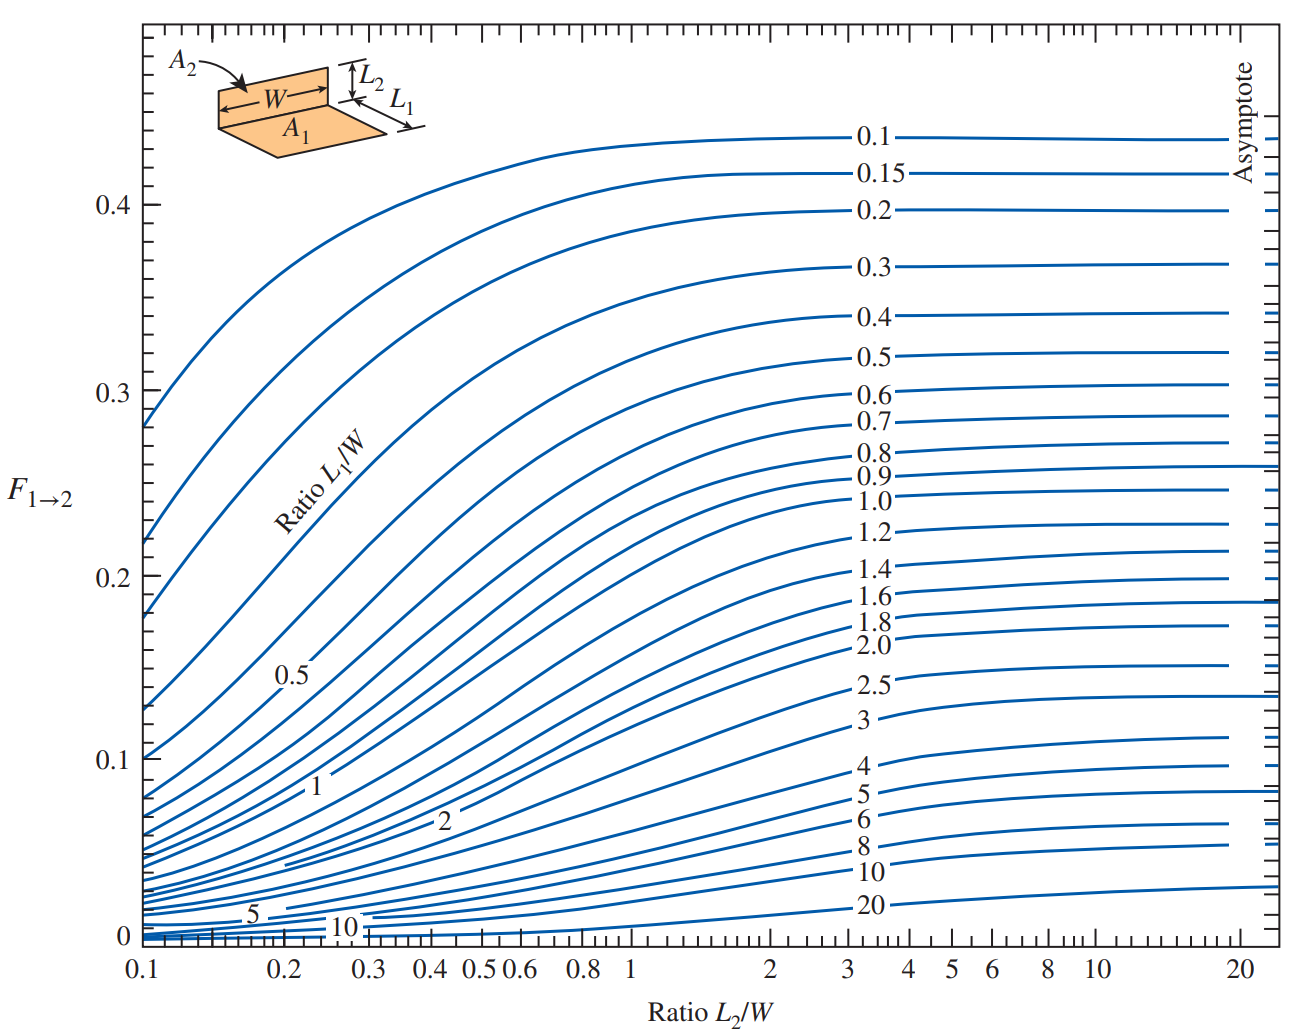
\includegraphics[width=0.6\textwidth]{Figures/Sec13 perpendicular rectangle.png}
    \caption{View factor between two perpendicular rectangles with a common edge}
    \label{fig:sec13_perpendicular_rectangles}
\end{figure}
\begin{figure}[H]
    \centering
    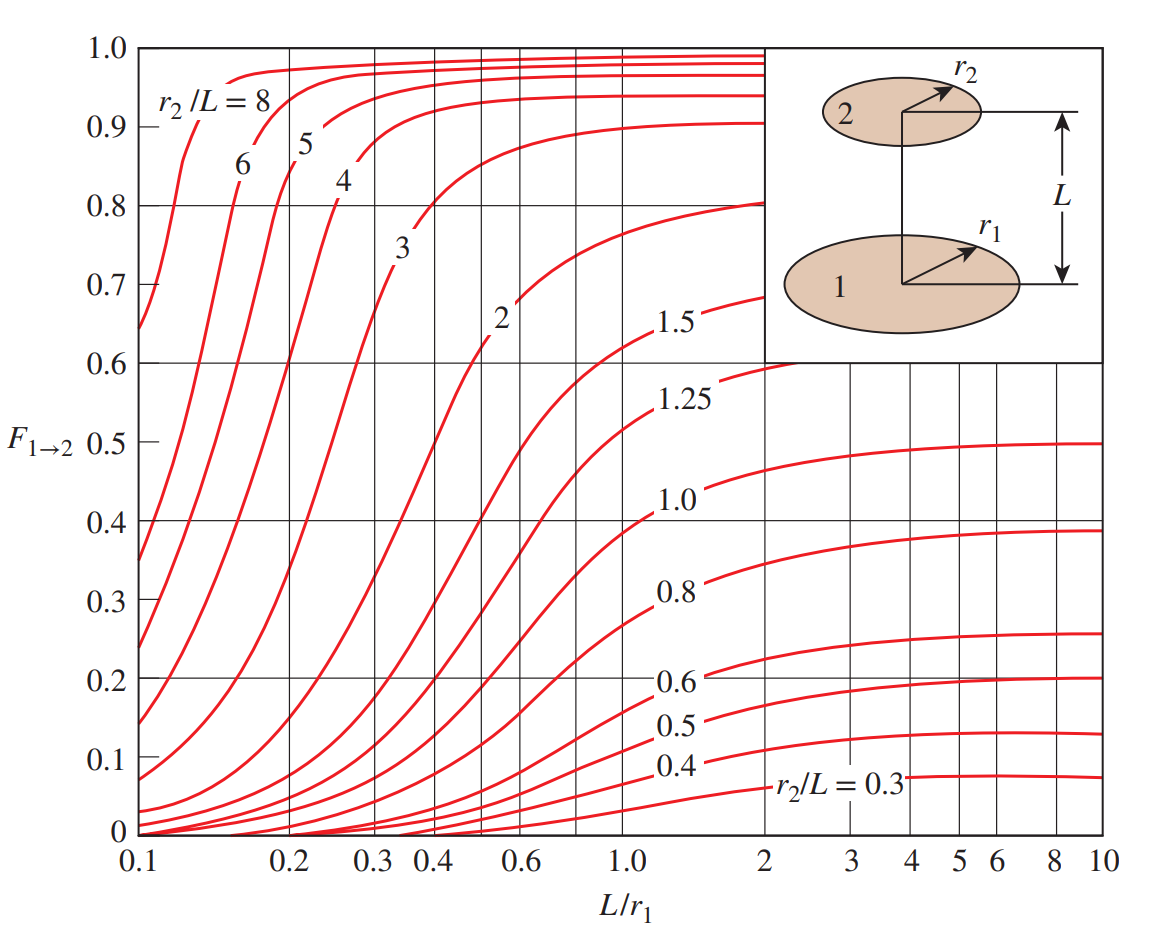
\includegraphics[width=0.6\textwidth]{Figures/Sec13 coaxial parallel disk.png}
    \caption{View factor between two coaxial parallel disks}
    \label{fig:sec13_coaxial_parallel_disks}
\end{figure}
\begin{figure}[H]
    \centering
    \begin{subfigure}[b]{0.4\textwidth}
        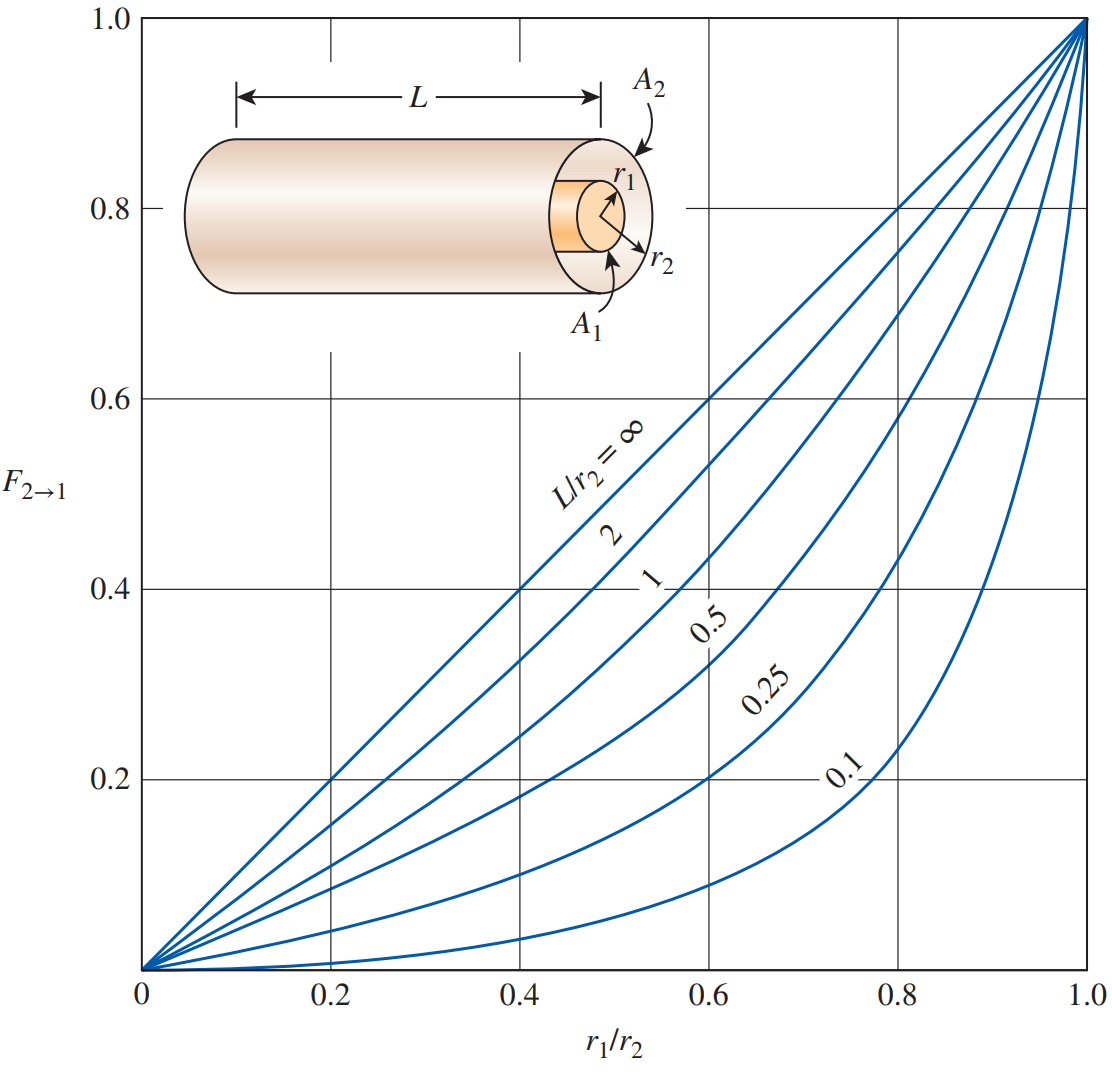
\includegraphics[width=\textwidth]{Figures/Sec13 concentric 2-1.png}
    \end{subfigure}
    \begin{subfigure}[b]{0.4\textwidth}
        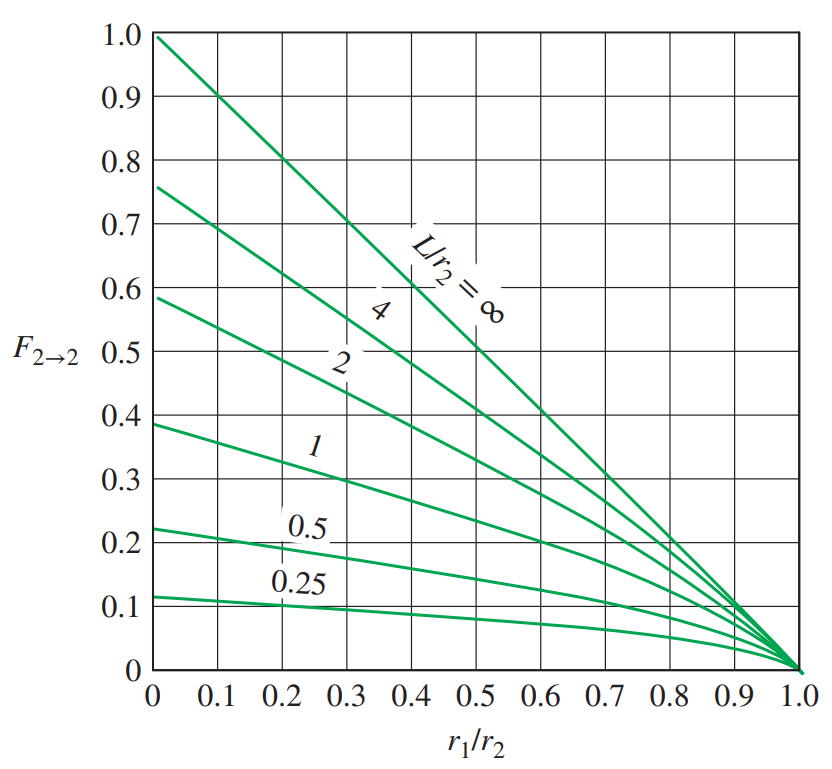
\includegraphics[width=\textwidth]{Figures/Sec13 concentric 2-2.png}
    \end{subfigure}
    \caption{View factors for two concentric cylinders of finite length: (a) outer cylinder to inner cylinder; (b) outer cylinder to itself.}
    \label{fig:sec13_concentric_cylinders}
\end{figure}

\section*{Tables}
\begin{table}[H]
    \centering
    \caption{Radiation heat transfer relations for some familiar two-surface arrangements}
    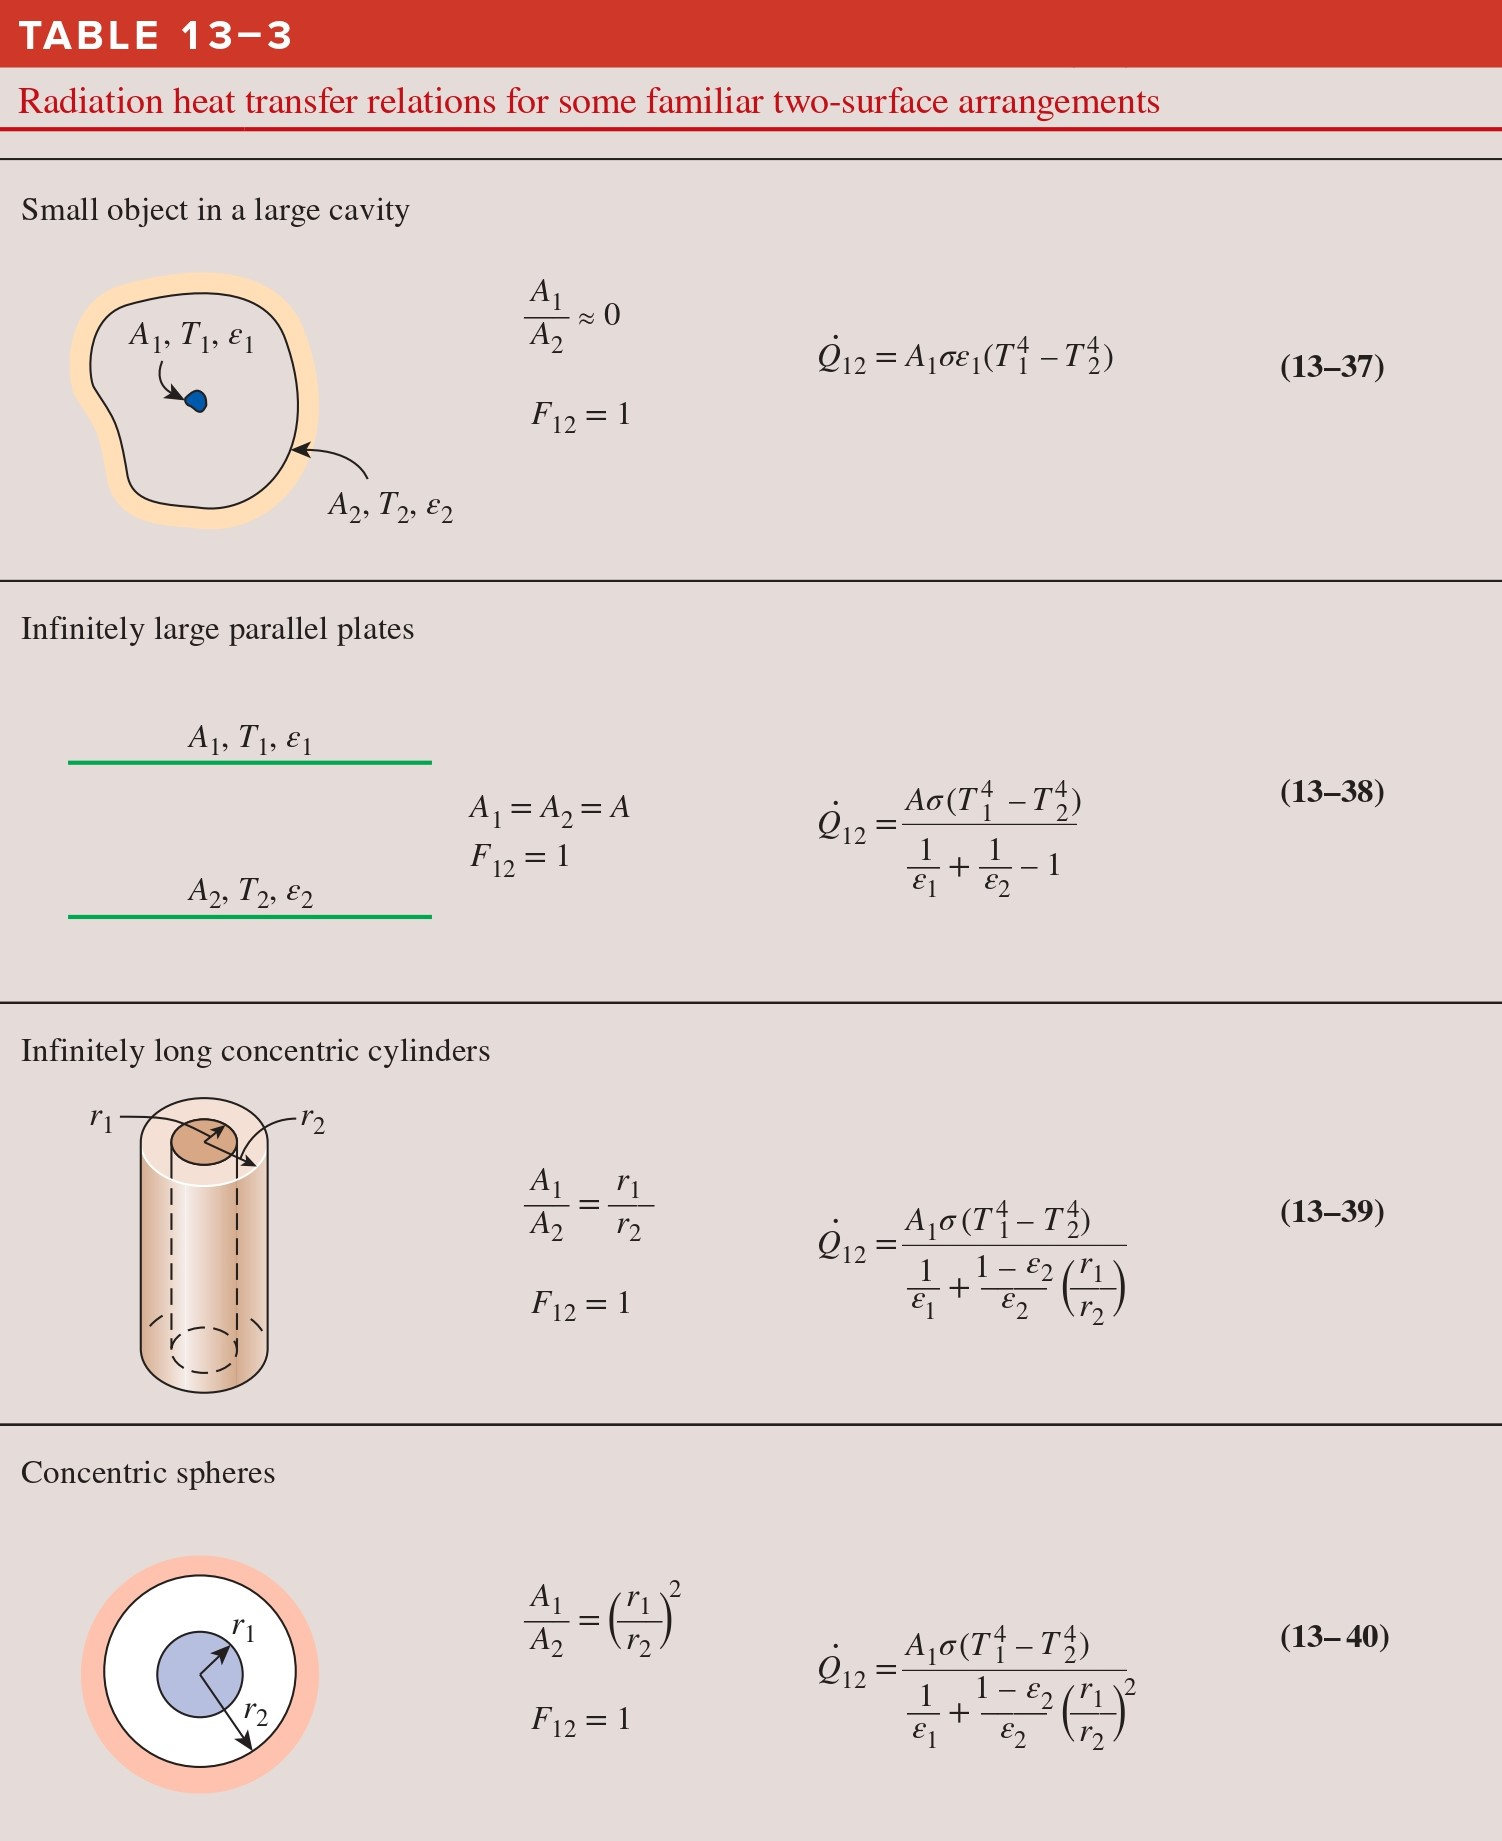
\includegraphics[width=0.8\textwidth]{Figures/Sec13 heat transfer enclosed.png}
    \label{tab:sec13_radiation_enclosure_relations}
\end{table}